%%% Preamble
\documentclass{report}

\usepackage[utf8]{inputenc}
\usepackage[T1]{fontenc}
\usepackage{fourier}
\usepackage[french]{babel}
\usepackage[protrusion=true,expansion=true]{microtype}	
\usepackage{amsmath,amsfonts,amsthm} % Math packages
\usepackage[pdftex]{graphicx}	
\usepackage{url}
\usepackage{pdfpages}
\usepackage{todonotes}
\usepackage[a4paper, body={16cm,26cm}]{geometry}
\usepackage{float}
\usepackage{framed}
\usepackage[toc,page]{appendix} 
\usepackage{multicol}
\usepackage{colortbl}
\usepackage{epstopdf}
\usepackage{adjustbox}

%%% Custom sectioning
\usepackage{sectsty}
\allsectionsfont{  \normalfont\scshape}
%\allsectionsfont{\centering \normalfont\scshape}

%%% Custom headers/footers (fancyhdr package)
\usepackage{fancyhdr}
\pagestyle{fancyplain}
\fancyhead{}								% No page header
\fancyfoot[L]{}							% Empty 
\fancyfoot[C]{}							% Empty
\fancyfoot[R]{\thepage}					% Pagenumbering
\renewcommand{\headrulewidth}{0pt}		% Remove header underlines
\renewcommand{\footrulewidth}{0pt}		% Remove footer underlines
\setlength{\headheight}{13.6pt}


%%% Equation and float numbering
\numberwithin{equation}{section}		% Equationnumbering: section.eq#
\numberwithin{figure}{section}		% Figurenumbering: section.fig#
\numberwithin{table}{section}		% Tablenumbering: section.tab#


%%% Define new commands
\newcommand{\horrule}[1]{\rule{\linewidth}{#1}} 	% Horizontal rule
\renewcommand{\bf}[1]{\textbf{#1}}
\renewcommand{\it}[1]{\textit{#1}}
\newcommand{\bfit}[1]{\textbf{\textit{#1}}}
\renewcommand{\sc}[1]{\textsc{#1}}

\newcommand{\Todo}[1]{\todo[inline]{#1}}
\renewcommand{\thesection}{\thepart .\arabic{section}}

\usepackage{tocloft}
\cftsetindents{chapter}{0em}{1em}
\cftsetindents{section}{1.5em}{2.5em}
\makeatletter
\def\l@figure{\@dottedtocline{1}{1.5em}{4em}}
\makeatother

\usepackage{bookmark}
%\usepackage[hidelinks]{hyperref}
\usepackage{cases}
\usepackage{color}
\usepackage{xcolor}
\usepackage{relsize}
\usepackage{caption}
\colorlet{shadecolor}{black!10}

\delimitershortfall-1sp
\newcommand\abs[1]{\left|#1\right|}


\usepackage{tikz, pgfplots}


%}}}
%{{{ --- pgfplots ---------------------

%{{{ Colors

% TolColors from http://www.r-bloggers.com/the-paul-tol-21-color-salute/
\definecolor{TolColor1}{HTML}{332288}   % dark purple
\definecolor{TolColor2}{HTML}{6699CC}   % dark blue
\definecolor{TolColor3}{HTML}{88CCEE}   % light blue
\definecolor{TolColor4}{HTML}{44AA99}   % light green
\definecolor{TolColor5}{HTML}{117733}   % dark green
\definecolor{TolColor6}{HTML}{999933}   % dark brown
\definecolor{TolColor7}{HTML}{DDCC77}   % light brown
\definecolor{TolColor8}{HTML}{661100}   % dark red
\definecolor{TolColor9}{HTML}{CC6677}   % light red
\definecolor{TolColor10}{HTML}{AA4466}  % light pink
\definecolor{TolColor11}{HTML}{882255}  % dark pink
\definecolor{TolColor12}{HTML}{AA4499}  % light purple

%}}}
%{{{ Color cycles

\pgfplotscreateplotcyclelist{mbarplot cycle}{%
  {draw=TolColor2, fill=TolColor2!70},
  {draw=TolColor7, fill=TolColor7!70},
  {draw=TolColor4, fill=TolColor4!70},
  {draw=TolColor11, fill=TolColor11!70},
  {draw=TolColor1, fill=TolColor1!70},
  {draw=TolColor8, fill=TolColor8!70},
  {draw=TolColor6, fill=TolColor6!70},
  {draw=TolColor9, fill=TolColor9!70},
  {draw=TolColor10, fill=TolColor10!70},
  {draw=TolColor12, fill=TolColor12!70},
  {draw=TolColor3, fill=TolColor3!70},
  {draw=TolColor5, fill=TolColor5!70},
}

\pgfplotscreateplotcyclelist{mlineplot cycle}{%
  {TolColor2, mark=*, mark size=1.5pt},
  {TolColor7, mark=square*, mark size=1.3pt},
  {TolColor4, mark=triangle*, mark size=1.5pt},
  {TolColor6, mark=diamond*, mark size=1.5pt},
}


\pgfplotsset{
  compat=1.9,
  mbaseplot/.style={
    legend style={
      draw=none,
      fill=none,
      cells={anchor=west},
    },
    x tick label style={
      font=\footnotesize
    },
    y tick label style={
      font=\footnotesize
    },
    legend style={
      font=\footnotesize
    },
    major grid style={
      dotted,
    },
    axis x line*=bottom,
  },
  mlineplot/.style={
    mbaseplot,
    xmajorgrids=true,
    ymajorgrids=true,
    major grid style={dotted},
    axis x line=bottom,
    axis y line=left,
    legend style={
      cells={anchor=west},
      draw=none
    },
    cycle list name=mlineplot cycle,
  },
  mbarplot base/.style={
    mbaseplot,
    bar width=6pt,
    axis y line*=none,
  },
  mbarplot/.style={
    mbarplot base,
    ybar,
    xmajorgrids=false,
    ymajorgrids=true,
    area legend,
    legend image code/.code={%
      \draw[#1] (0cm,-0.1cm) rectangle (0.15cm,0.1cm);
    },
    cycle list name=mbarplot cycle,
  },
  horizontal mbarplot/.style={
    mbarplot base,
    xmajorgrids=true,
    ymajorgrids=false,
    xbar stacked,
    area legend,
    legend image code/.code={%
      \draw[#1] (0cm,-0.1cm) rectangle (0.15cm,0.1cm);
    },
    cycle list name=mbarplot cycle,
  },
  disable thousands separator/.style={
    /pgf/number format/.cd,
      1000 sep={}
  },
}


%%  ========   IMPORTANT ========
%% Spécifier ici les variables pour le document
\newcommand{\mainTitle}{\'Etude préalable - SPIE}
\newcommand{\secondTitle}{Dossier d'Initialisation}
\newcommand{\documentRef}{DI/4401/1}

%%% Begin document
\begin{document}
%----------------------------------------------------------------------------------------
%	PACKAGES
%----------------------------------------------------------------------------------------

\documentclass[12pt]{article}
\usepackage[a4paper]{geometry}
\geometry{verbose,tmargin=1in,bmargin=0in,lmargin=1in,rmargin=1in}
\usepackage[utf8]{inputenc}
\usepackage[francais]{babel}
\usepackage[T1]{fontenc}

\usepackage{graphicx}
\begin{document}

\begin{titlepage}

\newcommand{\HRule}{\rule{\linewidth}{0.5mm}} % horizontal lines

\center % Center everything
 
%----------------------------------------------------------------------------------------
%	HEADING SECTIONS
%----------------------------------------------------------------------------------------

\vspace*{1cm}

\textsc{\LARGE INSA de LYON}\\[1.5cm] 
\textsc{\Large D\'epartement Informatique}\\[0.5cm] 
\textsc{\large Projet Longue Durée}\\[0.5cm] % 

%----------------------------------------------------------------------------------------
%	TITLE SECTION
%----------------------------------------------------------------------------------------

\HRule \\[0.4cm]
{ \huge \bfseries Compte Rendu}\\[0.1cm]
{\large \bfseries - Gestion des contacts commerciaux d'une banque -} 
\HRule \\[1.5cm]
 
%----------------------------------------------------------------------------------------
%	DATE SECTION
%----------------------------------------------------------------------------------------

{\large \today}\\[2cm] % 
 
%----------------------------------------------------------------------------------------
%	AUTHOR SECTION
%----------------------------------------------------------------------------------------

\begin{minipage}{0.4\textwidth}
\begin{center} \large
\emph{Auteurs} \\
Lisa \textsc{Courant} \\
Estelle \textsc{Lepeigneux} \\
Pierre \textsc{Jarsaillon} \\
Hugues \textsc{Verlin} \\
\end{center}
\end{minipage}
~
\begin{minipage}{0.4\textwidth}
\begin{center} \large
\emph{Chef de projet} \\
Paul \textsc{Dautry}
\end{center}
\begin{center} \large
\emph{Responsable Qualité} \\
Antoine \textsc{Chabert}
\end{center}
\end{minipage}\\[5cm]

H4401\\[2cm]

%----------------------------------------------------------------------------------------
%	LOGO SECTION
%----------------------------------------------------------------------------------------

\includegraphics[scale=0.3]{figures/logo.png}
%----------------------------------------------------------------------------------------

\vfill % Fill the rest of the page with whitespace

\end{titlepage}
\end{document}


%% Commenter les deux lignes suivantes pour le document final
%\listoftodos
%\newpage

%% Table de matière / figures / tableaux
\tableofcontents
\listoffigures
%\listoftables
\newpage

%% Faire une nouvelle partie :
%\part{NOM DE LA PARTIE}
%\setcounter{section}{0}
%\section{NOM DU CHAPITRE / SECTION}
%\subsection{NOM DU SOUS-CHAPITRE / SOUS-SECTION}

%% Inclure un document LaTeX :
%\input{file}

%% Inclure une figure :
%\begin{figure}[H]
%    \label{fig-LABEL-DE-LA-FIGURE}
%    \noindent\makebox[\textwidth]{\includegraphics[width=10cm]{figures/NOM-DE-LA-FIGURE.png}}
%    \caption{TEXTE DE LA LEGENDE}
%\end{figure}

% ------------------ Première partie : contexte -----------------
\part{Objet et contexte du projet}
\setcounter{section}{0}
\section{Objet du projet}

À l'origine de ce projet, une entreprise spécialisée dans les domaines de l'énergie, de la mécanique et des réseaux de communication : Spie. Son souhait ? Rendre son activité de « gestion des contrats de maintenance » plus homogène, afin que tous les aspects de son métier respectent un processus similaire. Mais le besoin de Spie ne s'arrête pas ici : la société s'oriente de plus en plus vers le secteur des énergies vertes, et ce domaine commence à faire partie intégrante de l'entreprise. Il faut donc qu'ici aussi le processus de maintenance des équipements industriels liés à ce nouveau secteur soit homogène à tous les autres processus de la société, tout comme il faut que n'importe quel nouveau secteur auquel Spie souhaiterait se consacrer soit un besoin facilement intégrable. Notre projet doit donc s'inscrire dans une démarche de globalisation, dans le but de rendre les activités de la société moins hétérogènes. \\
    
Sur un marché où tout va toujours plus vite, une telle demande d'homogénéisation ne semble pas incongrue, puisque cela permettra à Spie d'améliorer grandement son efficacité dans toute l'étape de maintenance des équipements. Cela facilitera également la compréhension des intervenants puisque les processus seront plus simples à appréhender et également similaires les uns aux autres : les utilisateurs seront donc beaucoup plus polyvalents.

\section{Contexte du projet}

Notre étude se positionne en réalité dans un projet de bien plus grande ampleur : en effet, nous nous limiterons ici à l'étude préalable, qui en est la toute première étape. L'objectif final de ce projet sera de proposer deux solutions permettant d'améliorer les processus de maintenance, qui devront impérativement prendre en compte les retours d'expérience que nous avons pu recevoir. Nous ne nous intéresserons pas à la suite de ce projet, mais allons plutôt nous assurer que nous exprimons les besoins de manière fonctionnelle et non en terme de solutions. L'analyse ainsi effectuée nous permettra de dégager toutes les fonctionnalités nécessaires à la réalisation d'un projet futur, en mettant au point un document définissant fonctionnellement le besoin, indépendamment d'une solution technique. \\
    
Pour ce faire, nous allons mettre en oeuvre certaines techniques de production, incluant la spécification de solutions informatiques, la mise en place de méthodes de conception ou encore l’élaboration d’un Plan d’Assurance Qualité. En constituant des équipes dont les rôles de chacun sont bien définis et répartis selon les compétences de chaque personne, nous pourrons organiser notre projet de la meilleure façon possible et proposer le suivi de l’avancement du projet en temps réel.


% ------------------ Seconde partie : livrables -----------------
\part{Descriptif des livrables du projet}
\setcounter{section}{0}
\let\cleardoublepage\clearpage
\section{Tableau des livrables}

\vspace{-1cm}
\begin{figure}[H]
\noindent\makebox[\textwidth]{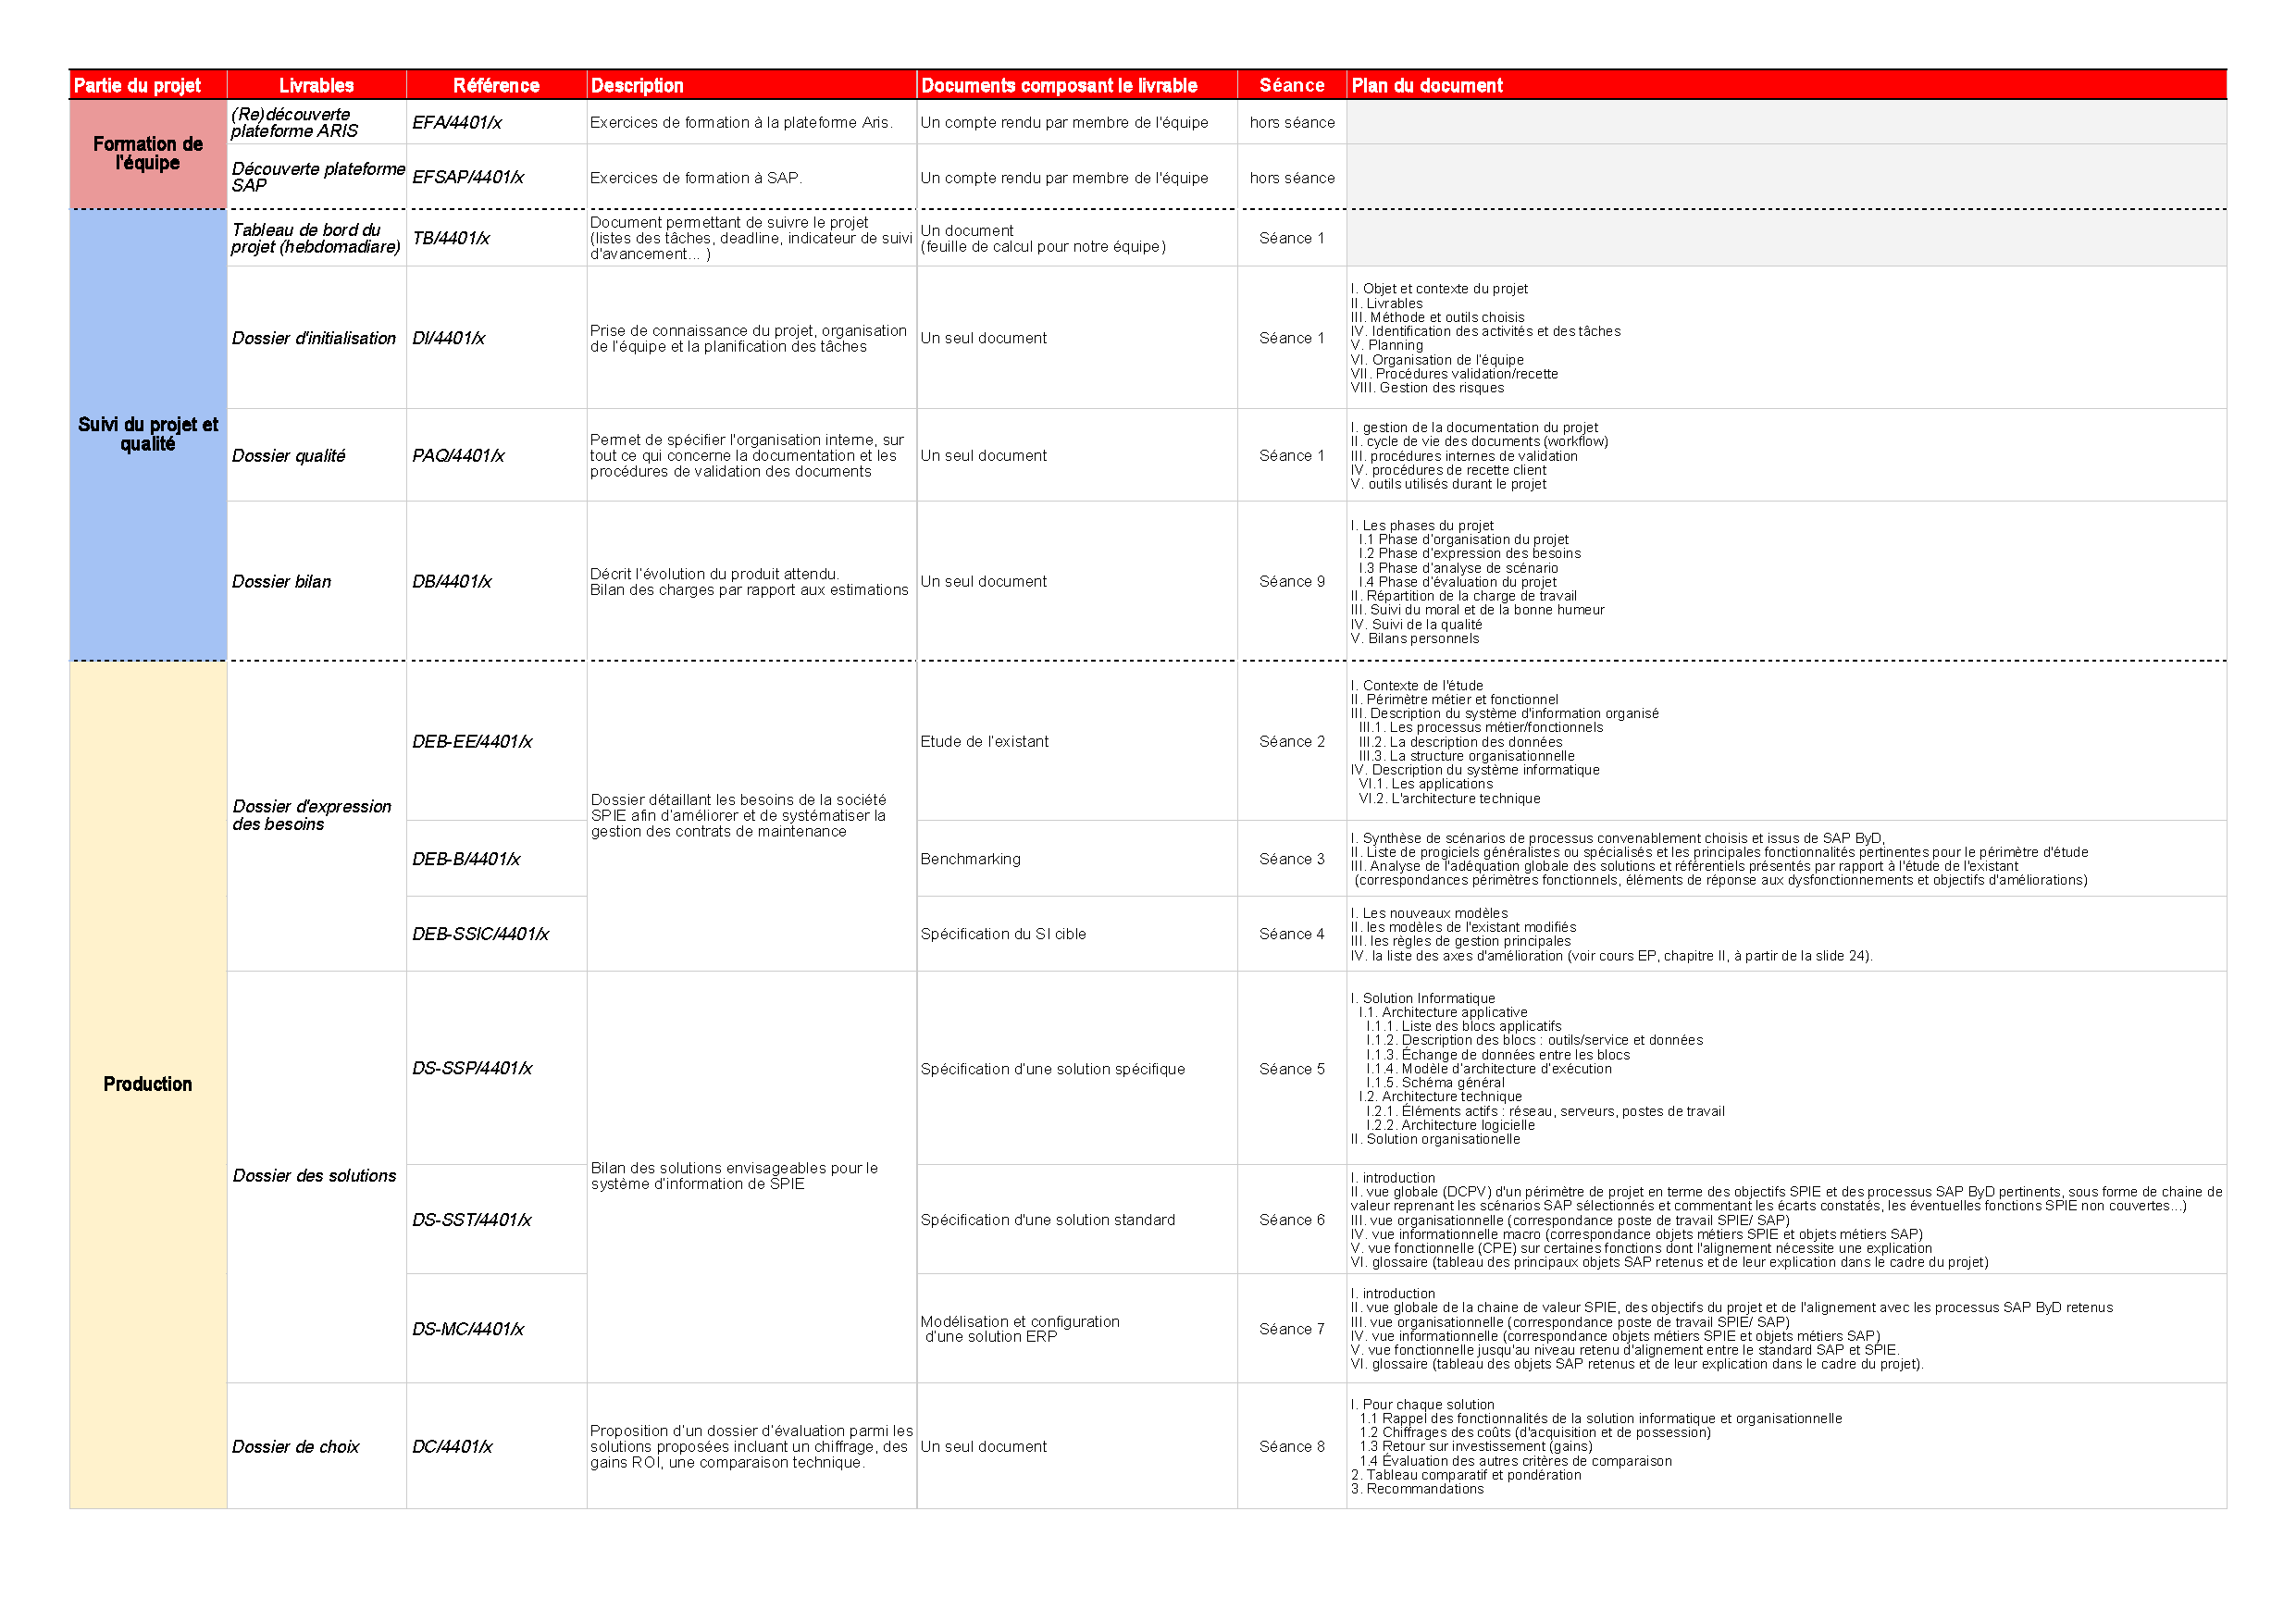
\includegraphics[width=21cm,angle=90]{figures/livrables.pdf}}
\caption{Tableau récapitulatif des livrables}
\end{figure}

\section{Description des documents attendus par phase du projet}

Cette partie permet de récapituler l’ensemble des livrables à remettre lors de chaque phase du projet, en présentant de manière synthétique leurs contenus. \\

Pour les plans de chaque document, il est nécessaire de se référer au tableau récapitulatif de chaque livrable.

\subsection{Phase d’initialisation}

\subsubsection{Le dossier d’initialisation}

Il s’agit du présent document. Son objectif est de décrire le but du projet, ainsi que son contexte en terme d’objectifs, de périmètre, d’acteurs. On y trouve également la description ci-présente des livrables. Le mode opératoire et les outils choisis y sont également définis.  \\

Ce document permet également l’identification des différentes activités et tâches, de façon à élaborer un planning du projet. \\

Enfin, il contient tous les éléments concernant notre équipe, tant en terme d’organisation qu’en terme de gestion des risques.

\subsubsection{Le PAQ}

Le PAQ ou Plan d’Assurance Qualité permet de décrire la façon dont notre équipe s’organise pour produire les livrables attendus avec la meilleure qualité qui soit. \\

Ainsi, on retrouve tout ce qui concerne la gestion de la documentation du projet et le cycle de vie des documents produits. Notre processus de validation interne est documenté, de même que les procédures de recette client. \\

Enfin, il liste l’ensemble des outils utilisés durant le projet et explicite le rôle de chacun de ces derniers dans le projet, c’est-à-dire l’exploitation que l’équipe fera de ces outils.

\subsubsection{Tableau de bord du projet (hebdomadiare)}

Une description avec des captures d’écran du tableau de bord permettant le suivi de projet sera remise avec le dossier d’initialisation. Le tableau de bord doit à tout instant donner une image fiable de l’avancement du projet et doit permettre de suivre ce dernier de manière fine afin de détecter toute irrégularité tel qu’un glissement au niveau du planning ou une chute du moral global de l’équipe.

\subsection{Phase de formation}

\subsubsection{(Re)Découverte de la plateforme ARIS}

Chaque membre de l’équipe doit rendre un compte rendu de 2 pages sur son ressenti lors de l’initiation qui consiste en la réalisation d’un exercice ARIS simple.

\subsubsection{Découverte plateforme SAP}

Chaque membre de l’équipe doit rendre un compte rendu de 2 pages sur son ressenti lors de l’initiation.

\subsection{Phase d’expression des besoins}

\subsubsection{Étude de l'existant}

Le but de ce rapport est de documenter l’organisation existante au sein de SPIE selon trois grands axes, qui sont l’axe fonctionnel, l’axe organisationnel et l’axe informatique, afin d’en établir les avantages et les inconvénients.\newline
Le rapport doit comporter environ une dizaine de pages.

\subsubsection{Benchmark}

Ce livrable peut s'appuyer sur des modèles ARIS. Ce rapport intermédiaire doit comprendre : \\

\begin{description}
    \item[\textbullet] Un résumé des scenarii des processus correctement élu depuis SAP ByD.
    \item[\textbullet] Un listing de progiciels avec des fonctionnalités intéressantes dans le cadre de l’étude.
    \item[\textbullet] Vérification de la conformité des solutions développées par rapport à l’existant.
\end{description}

\subsubsection{Spécification du SI cible}

Il s’agit ici de fournir un rapport intermédiaire concernant la modélisation en utilisant le formalisme ARIS. Ce rapport contiendra notamment : \\
\begin{description}
    \item[\textbullet] Les nouveaux modèles,
    \item[\textbullet] les modèles de l'existant modifiés,
    \item[\textbullet] les règles de gestion principales,
    \item[\textbullet] et la liste des axes d'amélioration.
\end{description}

\subsection{Phase : Dossier des solutions}

\subsubsection{Spécification d’une solution spécifique}

Les spécifications se présenteront sous la forme d’un rapport qui documente les dimensions fonctionnelle, organisationnelle et informatique de la solution.

\subsubsection{Spécification d’une solution standard}

La spécification de la solution standard comprend : \\
\begin{description}
    \item[\textbullet] La description de la solution standard à l’aide de modèle correspond aux besoins de SPIE, incluant le référentiel SAP ByD de manière à voir les enjeux organisationnels
    \item[\textbullet] L’ensemble des scénarii SAP sélectionnés
    \item[\textbullet] Enfin, il contiendra :
        \begin{description}
            \item[\textbullet] les matrices ARIS montrant l’accord entre les processus élaborées par notre équipe et ceux de SPIE,
            \item[\textbullet] les fonctions SAP,
            \item[\textbullet] et l’organigramme de SPIE.
        \end{description}
\end{description}

\subsubsection{Modélisation et configuration de la solution ERP}

Il s’agit à nouveau d’un rapport généré par ARIS qui contiendra : \\

\begin{description}
    \item[\textbullet] Les modèles permettant de décrire la solution standard répondant aux besoins de SPIE avec le standard SAP ByD, a un niveau suffisant pour permettre le dimensionnement du projet, 
    \item[\textbullet] la configuration des scénarii SAP sélectionnés,
    \item[\textbullet] et des matrices ARIS montrant l’accord entre les processus élaborés par notre équipe, et ceux de SPIE.
\end{description}

\subsection{Phase : Bilan}

\subsubsection{Évaluation des solutions}

Il s’agit ici de remettre \bf{un dossier de choix}. Celui doit mettre en avant les forces et faiblesses de chaque solution proposée par notre équipe.

\subsubsection{Restitution}

La restitution finale est constitué de deux livrables. On trouve : \\

\begin{description}
    \item[\textbullet] Une présentation
    \item[\textbullet] Un dossier bilan \\
\end{description}

Ces deux livrables auront pour but de donner l’ensemble des éléments quantitatifs concernant le projet, de manière à détailler les compétences acquises sous la forme d’un tableau.

% ------------------ Troisième partie : méthodes et outils -----------------
\part{Méthodes et Outils choisis}
\setcounter{section}{0}

\section{Présentation de la méthodologie}

Ce projet de grande envergure s’étale sur une durée de 12 semaines durant lesquelles des rendus intermédiaires seront effectués. Cela permet de pouvoir suivre l’avancement du travail et des différentes étapes de ce dernier. Il s’inscrit dans un processus méthodologique bien précis, découpé en grandes phases elles-mêmes découpées en sous-phases. Cette méthodologie est essentielle car elle suit une logique de conception centrale pour la bonne réalisation de ce projet.

\section{Détail par phase}

\subsection{Phase 1 : Initialisation du projet}

Cette première phase occupe les deux premières semaines du projet. Elle consiste en la réalisation des premiers rendus intermédiaires, c’est-à-dire le PAQ et le dossier d’initialisation. De ce fait, les objectifs sont principalement de déterminer les éléments importants à mettre en place dès le début du projet pour la bonne cohérence des différents documents organisationnels que nous allons produire. \\

Il faut aussi avoir une première connaissance et définition du métier et du périmètre fonctionnel sur lequel porte ce projet, et donc sur lequel portera toute l’étude, permettant une transition vers l’expression des besoins. Cette première étape permet au client de prendre connaissance de la manière avec laquelle nous procédons, notre organisation et toute autre information importante relative à la manière dont le projet sera conduit.

\subsection{Phase 2 : Expression des besoins}

Cette phase est la phase la plus importante. Elle permet de comprendre les différents aspects, à la fois fonctionnels, mais aussi techniques, du métier et du besoin qui a mené à la demande à laquelle ce projet tente de répondre. En effet, la première étape de cette phase est d’abord de se plonger au c\oe{}ur du métier et des processus qui sont actuellement mis en place au sein de l’entreprise, afin d’en comprendre toutes les facettes. Nous devons parvenir à identifier l’ensemble des objets et le domaine d’application, ainsi qu’à comprendre et maîtriser ces derniers. À l’aide d’outils de modélisation ARIS tels que ARIS Architect, disponible sur la plateforme ARIS mise à notre disposition par le client, nous pourrons identifier, formaliser et détailler ces processus et les acteurs impliqués sous forme de diagrammes BPM. \\

Dans un deuxième temps il sera question de comprendre les nouveaux besoins du client par rapport à l’existant. Cette étape pourra se dérouler sous forme de groupes de travail ou de réunions.

\subsection{Phase 3 : Élaboration des solutions}

Suite à l’expression des besoin dans laquelle nous aurons identifié l’existant en détail ainsi que les différentes attentes client vis-à-vis du nouveau SI en projet, il nous faudra définir plusieurs solutions à proposer en réponse au besoin et exigences du client. Deux solutions sont à définir, une reposant sur un ERP, et une autre plus classique, dans la continuité du SI existant.

\subsection{Phase 4 : Recommandations sur les solutions}
 
Dans cette phase, notre travail consistera en la critique des différentes solutions proposées par l’équipe et l’apport de conseils au client. L’idée étant de rendre la prise de décision plus aisée pour le client en lui fournissant une critique constructive basée sur des critères précis et éventuellement définis avec ce dernier.

\subsection{Phase 4 : Restitution}

Phase essentielle et primordiale du projet, c’est le moment où nous devrons soumettre nos solutions au client. Il s'agira alors de  réussir à convaincre le client tout en montrant les différentes aspects de notre projet et le soin qui y a été apporté.

% ------------------ Quatrième partie : activites, taches et planning -----------------
\part{Activités, tâches et planning}
\setcounter{section}{0}

\section{Identification des activités}

Les activités qui seront menées sur le projet présentées ci-après seront triées par l’objectif auquel elles appartiennent. Ces activités seront menées par les différents collaborateurs de l’équipe indépendemment    de leur rôle dans le projet. Seul le responsable de la tache aura le rôle le plaçant naturellement comme expert sur cette tâche. Il est important de noter qu’un responsable de tâche n’est pas nécessairement celui qui la réalise mais plutôt celui qui s’assure que cette tache sera menée à bien dans le temps imparti. Il est également de sa responsabilité de faire remonter toute information concernant un risque de glissement au niveau du planning. \\
  
Les activités sont donc les suivantes :\\

Activités de production : \\

\begin{description}
    \item[\textbullet] Recherche, Exploration
    \item[\textbullet] Analyse, Exploitation
    \item[\textbullet] Rédaction, Synthèse
    \item[\textbullet] Mise en forme
    \item[\textbullet] Packaging
\end{description}

Activités de gestion de la qualité : \\

\begin{description}
    \item[\textbullet] Vérification, Validation
    \item[\textbullet] Vérifier que les procédures mises en place sur le projet sont respectées
\end{description}

Activités de gestion de projet : \\

\begin{description}
    \item[\textbullet] Suivi des indicateurs, analyse et synthèse
    \item[\textbullet] Planification des tâches
    \item[\textbullet] Suivi de l’avancement des tâches
    \item[\textbullet] Remise des livrables
    \item[\textbullet] Assister aux réunions et animer les réunion hebdomadaires
    \item[\textbullet] Mettre en place des actions correctives
\end{description}

\section{Identification des tâches}

Les tâches présentées dans la suite de ce document ont été identifiées comme les tâches nécessaires à la réalisation des livrables demandés et seront donc triées par phase. Ensuite ces tâches seront affectées au type d’activité auquel elle sont liées.  

\subsection{Phase 1 - Initialisation}

\begin{description}
% -------------------------------------------------------------- P
    \item[] \bf{Tâches de production}
        \begin{description}
            \item[\textbullet] \it{Réaliser le dossier d’initialisation}
                \begin{description}
                    \item[\textbullet] Rédiger de la section “Objet du projet et contexte”
                    \item[\textbullet] Rédiger de la section “Livrables”
                    \item[\textbullet] Rédiger de la section “Mode opératoire et Outils choisis”
                    \item[\textbullet] Rédiger de la section “Organisation de l’équipe”
                    \item[\textbullet] Rédiger de la section “Gestion des Risques”
                \end{description}
            \item[\textbullet] \it{Réaliser le PAQ}
                \begin{description}
                    \item[\textbullet] Rédiger de la section “Gestion de la documentation du projet”
                    \item[\textbullet] Rédiger de la section “Cycle de vie des documents”
                    \item[\textbullet] Rédiger de la section “Procédures internes de validation”
                    \item[\textbullet] Rédiger de la section “Procédures de recette client“
                    \item[\textbullet] Rédiger de la section “Outils utilisés”
                \end{description}
            \item[\textbullet] \it{Mettre en forme le tableau de bord}
            \item[\textbullet] \it{Convertir le dossier d’initialisation vers LaTeX}
            \item[\textbullet] \it{Convertir le PAQ vers la LaTeX}
            \item[\textbullet] \it{Packaging des livrables} \\
        \end{description}
% -------------------------------------------------------------- Q
    \item[] \bf{Tâches de gestion de la qualité}
        \begin{description}
            \item[\textbullet] \it{Valider le dossier d’initialisation}
                \begin{description}
                    \item[\textbullet] Valider la section “Objet du projet et contexte”
                    \item[\textbullet] Valider de la section “Livrables”
                    \item[\textbullet] Valider de la section “Mode opératoire et Outils choisis”
                    \item[\textbullet] Valider de la section “Organisation de l’équipe”
                    \item[\textbullet] Valider de la section “Gestion des Risques”
                \end{description}
            \item[\textbullet] \it{Valider le PAQ}
                \begin{description}
                    \item[\textbullet] Valider de la section “Gestion de la documentation du projet”
                    \item[\textbullet] Valider de la section “Cycle de vie des documents”
                    \item[\textbullet] Valider de la section “Procédures internes de validation”
                    \item[\textbullet] Valider de la section “Procédures de recette client“
                    \item[\textbullet] Valider de la section “Outils utilisés”
                \end{description}
            \item[\textbullet] \it{Valider le tableau de bord}
            \item[\textbullet] \it{Relecture du dossier après conversion}
            \item[\textbullet] \it{Relecture du PAQ après conversion} \\
        \end{description}
% -------------------------------------------------------------- GP
    \item[] \bf{Tâches de gestion de projet}
        \begin{description}
            \item[\textbullet] Identifier les tâches
            \item[\textbullet] Faire le planning
            \item[\textbullet] Assister à la réunion CdP
            \item[\textbullet] Assister à la réunion RQ
            \item[\textbullet] Valider l'ébauche de Gantt
            \item[\textbullet] Animer la réunion hebdomadaire avec l’équipe
        \end{description}
\end{description}

\subsection{Phase 2 - Dossier d’expression du besoin}

\begin{description}
% -------------------------------------------------------------- P
    \item[] \bf{Tâches de production}
        \begin{description}
            \item[\textbullet] \it{Réalisation de l'Etude de l'Existant}
                \begin{description}
                    \item[\textbullet] Analyse des processus de gestion des contrats de maintenance
                        \begin{description}
                            \item[\textbullet] Analyser selon le point de vue fonctionnement
                            \item[\textbullet] Analyser selon le point de vue organisation
                            \item[\textbullet] Analyser selon le point de vue architectures informatiques
                        \end{description}
                    \item[\textbullet] Synthétiser les analyses
                        \begin{description}
                            \item[\textbullet] Rédiger la section "Gestion des contrats de maintenance, fonctionnement"
                            \item[\textbullet] Rédaction de la section "Gestion des contrats de maintenance, organisation"
                            \item[\textbullet] Rédaction de la section "Gestion des contrats de maintenance, architectures informatiques"
                        \end{description}
                    \item[\textbullet] Réaliser les modèles ARIS
                        \begin{description}
                            \item[\textbullet] Réaliser les modèles ARIS correspondant à la section "Gestion des contrats de maintenance, fonctionnement"
                            \item[\textbullet] Réaliser les modèles ARIS correspondant à la section "Gestion des contrats de maintenance, organisation"
                            \item[\textbullet] Réaliser les modèles ARIS correspondant à la section "Gestion des contrats de maintenance, architectures informatiques"
                        \end{description}
                    \item[\textbullet] Convertir le dossier d’Etude de l’Existant en LaTeX
                    \item[\textbullet] Produire le rapport ARIS
                \end{description}
            \item[\textbullet] \it{Effectuer le Benchmark}
                \begin{description}
                    \item[\textbullet] Effectuer les recherches sur Internet concernant les processus formalisés (SAP)
                    \item[\textbullet] Synthétiser les recherches
                    \item[\textbullet] Conversion le document de synthèse en LaTeX
                \end{description}
            \item[\textbullet] \it{Spécifier le SI cible}
                \begin{description}
                    \item[\textbullet] Réaliser la modélisation des données
                    \item[\textbullet] Réaliser la modélisation des différents processus
                    \item[\textbullet] Rédiger le document de synthèse des modèles
                    \item[\textbullet] Rédiger du document de synthèse du modèle de données
                \end{description}
            \item[\textbullet] \it{Fusion des documents}
            \item[\textbullet] \it{Packaging des livrables}
        \end{description}
% -------------------------------------------------------------- Q
    \item[] \bf{Tâches de gestion de la qualité}
        \begin{description}
            \item[\textbullet] \it{Valider l’Etude de l’Existant}
                \begin{description}
                    \item[\textbullet] Valider la section "Gestion des contrats de maintenance, fonctionnement"
                    \item[\textbullet] Valider de la section "Gestion des contrats de maintenance, organisation"
                    \item[\textbullet] Valider de la section "Gestion des contrats de maintenance, architectures informatiques"
                \end{description}
            \item[\textbullet] \it{Valider les modèles ARIS}
                \begin{description}
                    \item[\textbullet] Valider les modèles ARIS correspondant à la section "Gestion des contrats de maintenance, fonctionnement"
                    \item[\textbullet] Valider les modèles ARIS correspondant à la section "Gestion des contrats de maintenance, organisation"
                    \item[\textbullet] Valider les modèles ARIS correspondant à la section "Gestion des contrats de maintenance, architectures informatiques"
                \end{description}
            \item[\textbullet] \it{Valider le Benchmark}
            \item[\textbullet] \it{Valider la spécification du SI cible}
                \begin{description}
                    \item[\textbullet] Valider la modélisation des données
                    \item[\textbullet] Valider la modélisation des différents processus
                    \item[\textbullet] Valider le document de synthèse des modèles
                    \item[\textbullet] Valider du document de synthèse du modèle de données
                \end{description}
            \item[\textbullet] \it{Relecture du l’Etude de l’Existant après conversion}
            \item[\textbullet] \it{Relecture des modèles ARIS après conversion}
            \item[\textbullet] \it{Relecture du Benchmark}
            \item[\textbullet] \it{Relecture de la spécification du SI cible}
        \end{description}
% -------------------------------------------------------------- GP
    \item[] \bf{Tâches de gestion de projet}
        \begin{description}
            \item[\textbullet] Animer les réunions hebdomadaires
            \item[\textbullet] Suivre les indicateurs
            \item[\textbullet] Entreprendre des actions correctives si nécessaire 
            \item[\textbullet] Rédiger les documents de suivi
        \end{description}
\end{description}

\subsection{Phase 3 - Dossier d'élaboration de solution}

\begin{description}
% -------------------------------------------------------------- P
    \item[] \bf{Tâches de production}
        \begin{description}
            \item[\textbullet] \it{Réaliser le dossier d'Elaboration de Solutions}
                \begin{description}
                    \item[\textbullet] Réaliser l'Etude de la solution spécifique
                        \begin{description}
                            \item[\textbullet] Concevoir la solution informatique
                            \item[\textbullet] Concevoir l’architecture applicative
                                \begin{description}
                                    \item[\textbullet] Lister les blocs applicatifs
                                    \item[\textbullet] Décrire les blocs : outils/service et données
                                    \item[\textbullet] Décrire les échange de données entre les blocs
                                    \item[\textbullet] Modéliser l’architecture d’exécution
                                    \item[\textbullet] Réaliser le schéma général
                                \end{description}
                    \item[\textbullet] Concevoir l’architecture technique
                        \begin{description}
                            \item[\textbullet] Lister les éléments actifs : réseau, serveurs, postes de travail
                            \item[\textbullet] Concevoir l’architecture logicielle
                        \end{description}
                    \item[\textbullet] Identifier les nouvelles données si nécessaire
                    \item[\textbullet] Concevoir la solution organisationnelle
                        \begin{description}
                            \item[\textbullet] Identifier les acteurs humains et leurs rôles
                            \item[\textbullet] Identifier les flux d'information
                        \end{description}
                    \item[\textbullet] Concevoir la solution fonctionnelle
                        \begin{description}
                            \item[\textbullet] Identifier les nouveaux processus
                        \end{description}
                \end{description}
                    \item[\textbullet] Réaliser l'Etude de la solution ERP
                        \begin{description}
                    \item[\textbullet] Réaliser le rapport ARIS
                        \begin{description}
                            \item[\textbullet] Rédiger de l'introduction
                            \item[\textbullet] Réaliser la vue globale (DCPV) d'un périmètre de projet en terme des objectifs SPIE et des processus SAP ByD pertinents
                            \item[\textbullet] Réaliser la vue organisationnelle 
                            \item[\textbullet] Réaliser la vue informationnelle macro
                            \item[\textbullet] Réaliser la vue fonctionnelle (CPE) sur certaines fonctions dont l'alignement nécessite une explication
                            \item[\textbullet] Rédiger le glossaire 
                        \end{description}
                \end{description}
                \end{description}
            \item[\textbullet] \it{Packager le dossier d'Elaboration de Solutions}
                \begin{description}
                    \item[\textbullet] Fusionner des rapports intermédiaires
                \end{description}
        \end{description}
% -------------------------------------------------------------- Q
    \item[] \bf{Tâches de gestion de la qualité}
        \begin{description}
            \item[\textbullet] \it{Valider l'Etude de la solution spécifique}
                \begin{description}
                    \item[\textbullet] Valider la solution informatique
                        \begin{description}
                            \item[\textbullet] Valider l'architecture applicative
                            \item[\textbullet] Valider l'architecture technique
                            \item[\textbullet] Valider les données identifiées
                        \end{description}
                    \item[\textbullet] Valider la solution organisationnelle
                    \item[\textbullet] Valider la solution fonctionnelle
                \end{description}
            \item[\textbullet] \it{Valider l'Etude de la solution ERP}
            \item[\textbullet] \it{Valider du rapport ARIS}
            \item[\textbullet] \it{Valider le dossier complet}
        \end{description}
% -------------------------------------------------------------- GP
    \item[] \bf{Tâches de gestion de projet}
        \begin{description}
            \item[\textbullet] Animer les réunions hebdomadaires
            \item[\textbullet] Suivre les indicateurs
            \item[\textbullet] Entreprendre des actions correctives si nécessaire 
            \item[\textbullet] Rédiger les documents de suivi
        \end{description}
\end{description}

\subsection{Phase 4 - Réalisation du dossier de choix}

\begin{description}
% -------------------------------------------------------------- P
    \item[] \bf{Tâches de production}
        \begin{description}
            \item[\textbullet] \it{Décrire de la solution spécifique}
                \begin{description}
                    \item[\textbullet] Rappeler les fonctionnalités de la solution informatique et organisationnelle
                    \item[\textbullet] Chiffrer les coûts (d'acquisition et de possession)
                    \item[\textbullet] Évaluer le retour sur investissement (gains)
                    \item[\textbullet] Évaluer les autres critères de comparaison
                \end{description}
            \item[\textbullet] \it{Décrire la solution ERP}
                \begin{description}
                    \item[\textbullet] Rappeler les fonctionnalités de la solution informatique et organisationnelle
                    \item[\textbullet] Chiffrer les coûts (d'acquisition et de possession)
                    \item[\textbullet] Évaluer le retour sur investissement (gains)
                    \item[\textbullet] Évaluer les autres critères de comparaison
                \end{description}
            \item[\textbullet] \it{Faire le tableau comparatif et pondération}
                \begin{description}
                    \item[\textbullet] Réaliser le tableau comparatif
                        \begin{description}
                            \item[\textbullet] Définir des critères de comparaison
                            \item[\textbullet] Remplir du tableau
                            \item[\textbullet] Rédiger de la synthèse du tableau
                            \item[\textbullet] Effectuer la recette du tableau
                        \end{description}
                \end{description}
        \end{description}
% -------------------------------------------------------------- Q
    \item[] \bf{Tâches de gestion de la qualité}
        \begin{description}
            \item[\textbullet] Valider la description de la solution spécifique
            \item[\textbullet] Valider la description de la solution ERP
            \item[\textbullet] Valider le tableau
        \end{description}
% -------------------------------------------------------------- GP
    \item[] \bf{Tâches de gestion de projet}
        \begin{description}
            \item[\textbullet] Animer les réunions hebdomadaires
            \item[\textbullet] Suivre les indicateurs
            \item[\textbullet] Entreprendre des actions correctives si nécessaire 
            \item[\textbullet] Rédiger les documents de suivi
        \end{description}
\end{description}

\subsection{Phase 5 - Préparation de la présentation}

\begin{description}
% -------------------------------------------------------------- P
    \item[] \bf{Tâches de production}
        \begin{description}
            \item[\textbullet] Préparer la présentation
            \item[\textbullet] Rédiger le dossier bilan
        \end{description}
\end{description}

\bf{Note concernant la plannification :} les deadlines et les temps alloués à chaque tâche sont décrits de manière exhaustive dans le Tableau de Bord concernant la page de suivi des tâches. Veuillez vous reporter à ce document pour tout complément d’information concernant l’aspect temporel des tâches identifiées précédemment et leur ordonnancement.

% ------------------ Cinquième partie : organisation equipe -----------------
\part{Organisation de l'équipe}
\setcounter{section}{0}
\section{Généralité}

Dans un premier temps, l’équipe va travailler comme un seul et même groupe. Puis, dans le but de mener au mieux ce projet, chacun aura un rôle spécifique et donc des responsabilités dans un domaine donné afin de paralléliser les tâches.

\section{Rôles}

\subsection{Chef de Projet}

Le chef de projet sera Paul Dautry.
Il assurera que le projet sera mené à bien et que son déroulement sera optimal. Toute l’équpe lui fera confiance afin qu’il identifie et redistribue les différentes tâches en fonction des compétences de chacun. Son rôle sera également de maintenir le tableau de bord à jour et d’établir le planning. En cas de dépassement des délais ou de mauvaise gestion de notre temps, il sera de son devoir de redresser la barre pour que le projet avance de façon rapide et efficace.

\subsection{Responsable Qualité}

Antoine Chabert sera notre responsable qualité : ce rôle non négligeable permettra à tous les documents du projet d’être cohérents, aussi bien du point de vue de la forme qu’au niveau du contenu. Des documents tels que le Plan d’Assurance Qualité répondent exactement à cette demande, permettant à tous nos livrables d’être homogènes.
    Il communiquera en permanence avec tous les membres de l’équipe afin d’assurer la justesse et la cohérence de leurs documents.

\subsection{Experts}

Enfin, plusieurs experts seronts assignés à différentes tâches du projet.

\subsubsection{Responsable modélisation/processus}

Estelle Lepeigneux sera responsable modélisation/processus. Ce responsable effectura de nombreuses démarches de conception, d’urbanisation et d’architecture d’entreprise. Il devra s’assurer que la refonte des processus de Spie est optimale et adaptée aux évolutions des métiers de l’entreprise. Il devra également garantir que les solutions construites répondent aux attentes organisationnelles et informatiques et suivent un modèle adapté et respectant les critères du processus de modélisation.

\subsubsection{Expert ERP}

Hugues Verlin sera expert ERP. Il aura la charge de contrôle la réalisation du modèle cible basé sur les fonctions standard SAP sélectionnées. Ledit modèle sera documenté afin de répondre au mieux aux besoins de Spie. L’expert devra veiller au respect des “bonnes pratiques”.

\subsubsection{Expert Métier}

L’expert métier sera Pierre Jarsaillon. Il fera bénéficier l’équipe de sa compétente fonctionnelle sur les processus métier lors de la mise en place de solutions sur l’amélioration et la maintenance du Système d’Information de Spie.

\subsubsection{Formateur ARIS}

Le formateur ARIS sera Lisa Courant. Le formateur s’assurera de la réalisation des modèles et livrables générés grâce à l’approche de modélisation ARIS. Son travail permettra de montrer l'adéquation entre les différents aspects du SAP et ceux de Spie.

Répartition des tâches
    Les responsabilités des tâches seront représentées sur la figure suivante.

\begin{figure}[H]
    \label{fig-risque}
    \noindent\makebox[\textwidth]{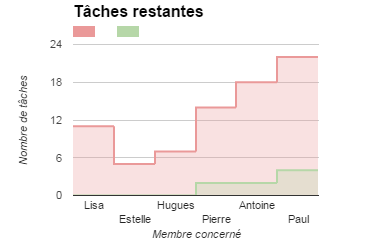
\includegraphics[width=10cm]{figures/taches_restantes.png}}
    \caption{Répartition des tâches par membres (responsabilités)}
\end{figure}

Le chef de projet et le responsable qualité ont un nombre de tâches légèrement supérieur du fait de leur statuts. Pour les autres membres du projet, le temps de travail a été réparti de la façon la plus équilibrée possible : certains responsables ont un peu plus de tâches, mais elles peuvent être plus rapides à effectuer que d’autres.

% ------------------ Sixième partie : procedures de validation et recette -----------------
\part{Procédures de validation et de recette}
\setcounter{section}{0}
Les procédures de validation et de recette sont décrite de manière détaillée dans le PAQ référencé PAQ/4401/1.
% ------------------ Première partie : livrables -----------------
\part{Gestion des risques}
\setcounter{section}{0}

\section{Généralités}

Au cours d’un projet de grande ampleur et de longue durée, nombre de facteurs externes et internes peuvent impacter le déroulement de celui-ci. Afin de limiter ces impacts, il est nécessaire de mettre en place une gestion des risques, qui devra permettre d’anticiper les situations à effet négatif sur le déroulement du projet. Pour cela, une démarche en quatre temps est mise en place, consistant à identifier dans un premier temps le risque. L’analyse de ce dernier est alors effectuée, afin de le classifier, estimer sa fréquence d’occurrence et estimer ses impacts. Cela permet par la suite de prévoir des plans de réponse en conséquence, qui pourront être appliqués lorsque la situation à risque surviendra. Enfin, la quatrième étape de suivi permet de contrôler de façon régulière la possible apparition du risque, en réalisant notamment des contrôles et des rapports de façon régulière. \\

\begin{figure}[H]
    \centering
    \label{fig-risque}
    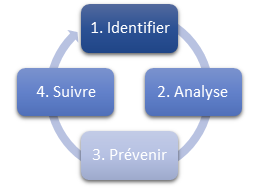
\includegraphics[scale=0.6]{figures/processus_risques.png}
    \caption{Processus de maîtrise des risques}
\end{figure}

Afin d’identifier les risques, il est nécessaire de déterminer dans un premier temps les différents facteurs qui peuvent les déclencher. Il faut cependant distinguer les facteurs humains des facteurs liés au projet, ces derniers étant spécifiques. \\

\section{Facteurs liés à l'humain}

En effet, d’un point de vue humain, la motivation de l’équipe est un facteur très important et ne doit pas être négligé, afin de conserver une productivité favorable. Au regard de la durée du projet, les diminutions de moral peuvent être jugées comme fort probables, et le chef de projet devra y remédier en discutant des problèmes avec son équipe. Afin de surveiller ce risque, un court entretien hebdomadaire personnalisé sera mis en place, au cours duquel les collaborateurs seront invités à noter leur humeur sur une échelle de 0 à 5 et à faire part de leurs remarques sur le déroulement du projet si besoin est. \\
 
Ce projet, de longue durée, devra également être conduit sur une période hivernale, qui augmente fortement le risque de maladie et, a fortiori, de baisse de productivité. Une répartition des tâches modulable est donc à prévoir, afin de permettre un transfert temporaire de productivité. \\
 
\section{Facteurs liés au projet}
 
Concernant les facteurs de risque liés au projet, les livrables devront être terminés dans les temps, afin de ne pas entraîner de glissement dans le planning et impacter d’autres collaborateurs du projet. Les risques de dépassement de délai, entraînant également un dépassement de budget, doivent donc être pris en compte. Afin de prévenir cette situation, les collaborateurs devront utiliser les moyens de communication mis à leur disposition pour signaler toute probabilité de dépassement lié à leurs activités. Ce signalement permettra de mettre en place le plan d’action permettant d’adapter le planning, notamment en réaffectant des collaborateurs en fonction de leur charge de travail. \\
 
Nous pouvons également noter un risque de dépassement des limites du projet, ce dernier étant dans un contexte pouvant porter à confusion, au regard du degré d’intégration de celui-ci. En effet, étant donné la complexité du projet, nombre d’interactions entre les différents acteurs sont à noter. Une étroite collaboration entre le responsable qualité et les autres collaborateurs est donc à prévoir, afin de surveiller la possible émergence de ces facteurs de risque. Le responsable qualité devra ainsi s’assurer que les travaux produits se limitent bien à l’apport de réponses concrètes et cohérentes aux besoins et aux demandes du client. \\

Enfin, l’estimation des temps nécessaires à la réalisation des tâches présente également un risque lié au projet. En effet, si cette étape n’est pas effectuée correctement, les risques de glissement présenteront une fréquence d’occurrence critique. Le manque d’expérience des collaborateurs concernant l’estimation des tâches à réaliser dans ce projet est un important facteur de risque. Afin de prévenir cette situation, l’estimation des durées nécessaires sera effectuée en se positionnant dans les pires cas. \\


%%% End document
\end{document}
